\documentclass[12pt]{article}
\usepackage[top=1in, bottom=1in, right=1in, left=1in]{geometry}
\usepackage{setspace}
\usepackage{graphicx}
\usepackage{setspace}
\usepackage{parskip}
\usepackage{url}

\title{Tough Choices: Excepted Service Appointments and the Presidential Allocation of Attention}
\date{April 9, 2015}
\author{Emily H. Moore \\ Washington University-Saint Louis}
\affil


\usepackage{Sweave}
\begin{document}
\Sconcordance{concordance:MooreToughChoicesTYP.tex:MooreToughChoicesTYP.Rnw:%
1 14 1 1 0 470 1}

\maketitle
\parindent=0.5in
\parskip=0.01in
\doublespacing

President Taft once said ``every time I make an appointment I create nine enemies and one ingrate'' (Pfiffner 2015). It takes millions of employees to run the federal bureaucracy and the difficult and often controversy-inspiring task of appointing several thousand of them rests with the president. The most visible of these are presidentially-appointed, Senate-confirmed positions. As Lewis and Waterman (2013) note, almost all studies focus on these high-profile personnel. Certainly, journalists have mainly studied appointees via the advice and consent process, but even scholars, who have broadened their scope beyond only traditional top level appointees have largely ignored lower level employees. Doing so misses an important part of administrative politics. 

Clearly Senate-confirmed appointees are important policymakers, but the president has a clear need for other types of employees as well, especially considering the increasing length of time to confirmation and the consequently shrinking amount of time these appointees serve. As Pfiffner points out, it took fewer than 2.5 months for John F. Kennedy's appointees to make it through the advice and consent process, but George Bush's appointees waited nearly nine months to begin serving. While Ronald Reagan managed to appoint 86 percent of the top appointees in his first year, Obama could not complete two-thirds. Partially as a result of this, the average time in office for these political appointees is only 2.5 years. It would seem ideal for all employees in the government, and particularly those with policy-making authority, to undergo a vetting process such as advice and consent, but the sheer volume of appointees and polarization in Congress quickly dissolves this notion. Clearly, the president requires a way to staff the bureaucracy quickly and with a certain amount of flexibility.

Thus, one of the president's key advantages as Administrator-in-Chief is his ability to hire low-level bureaucrats. These employees have considerable influence over policy and largely slip under the radar of congressional and media oversight (Lewis and Waterman 2013). This is partly because the president chooses who to appoint to these positions without congressional approval. Still, these appointments are perfectly legal exercises of presidential power with which Congress is complicit, and while low-level appointees certainly serve in political capacities, they also perform other functions. For example, appointees play an essential informational role which benefits both Congress and the president (Gailmard and Patty 2012). Additionally, appointees serve in a simple functional capacity, existing, in part, to help execute policy day-to-day. Clearly, as head of an ever-expanding administrative state, the president must also consider this practical aspect of the bureaucracy. Given finite resources to complete policy tasks (and particularly finite because only some appointments can be made wherever he wants them), how does the president choose to allocate his resources? On which agencies does he spend his time? 

Previous scholars have focused on how appointment power confers political control, but low-level employment patterns also provide information about the president's \textit{attentiveness} to a particular agency---an angle left unstudied in previous research. Yet attention is one of the president's most limited resources. Thus, students of bureaucracy should take note of how presidents allocate their administrative attention. While some research seeks to determine the degree of political appointees' loyalty or expertise in particular agencies (Lewis and Waterman 2013) or how the president chooses bureaucrats generally (Epstein and O'Halloran 1999; Lewis and Waterman 2013; Moe 1985), there is little work exploring how the president distributes his resources across the bureaucracy as a whole. 

In this paper, I use Schedule C and Excepted Service Executive Appointments to consider attention and politicization. First, I explore several expectations with regard to low-level appointees, studying the Department of Homeland Security and liaison agencies as cases. I also use a negative binomial regression model to explore the relationship between low-level personnel and presidential ideology. I then compare shares of appointees across and within the George W. Bush and Barack Obama presidencies. 

\section{Literature Review}
As a long history of literature suggests, presidents care about how agencies execute policy. Much scholarly work is devoted to the president's tradeoff between competent ``experts" and political loyalists (e.g. Hollibaugh forthcoming; Hollibaugh et al. forthcoming; Parsneau 2013). While the former cannot necessarily be trusted to advance the president's political interests (Moe 1985), the latter may lack the skill to execute policy well or efficiently (e.g. Lewis 2005; Gilmour and Lewis 2006; Heclo 1975, 1977). A related body of literature explores how presidents select appointees generally (e.g. Cohen 1988; Fenno 1959; Mackenzie 1981; Moe 1985) or conditionally based on the agency (Hollibaugh et al. forthcoming; Lewis and Waterman 2013). Others are concerned with the extent to which these positions are less policy oriented and more about patronage (e.g. Hollibaugh et al. forthcoming; Patterson 2008; Patterson and Pfiffner 2001; Tolchin and Tolchin 2010). Scholars have been particularly concerned with a tendency for the president to ``politicize" the bureaucracy (that is use appointees selected based on their ties to the party rather than expertise), which many argue is a more recent phenomenon (e.g. Burke 1992; Hart 1995; Heclo 1975; Lewis 2005, 2008; Wayne et al. 1979).

The appointment literature is couched within a larger framework of congressional-presidential relations. While many of the studies cited above are concerned with politicization because of its implications for bureaucratic performance, others are concerned with the president's propensity for unilateral action, which may be at odds with congressional wishes. Indeed, if not for political reasons, the bodies themselves may disagree about the bureaucratic system's institutiontal purpose (e.g. Lewis 2003). If that is the case, why would Congress allow the president such a long leash on his appointment powers? 

First, Congress has its own means of observing and reacting to executive actions (McCubbins and Schwartz 1984). More importantly, Congress has its own incentives to allow the president to appoint co-partisans to administrative positions. As Gailmard and Patty (2012) make clear, if the president is to have some control over the bureaucracy, Congress would at least like the indiviuals he appoints to be informed, even if the body is ideologically distant. Indeed, if Congress requires that agents use information as it would, ``Congress would simultaneously undermine the value of expertise to the bureaucrats in the first place" (130). Congress recognizes that some policy drift is inevitable. Faced with this predicament, it must choose whether or not it wants policy choices to be informed. Thus, Congress tolerates (even supports) the president's burgeoning administrative powers, going so far as to design the very intitutions which facilitate its loss of power. In light of this framework, Congress' willingness to allow the president greater control over both who he chooses to appoint and where he chooses to appoint them is brought into focus.  

While influence (both presidential on agency and agency on policy) is well-studied, there is virtually no literature considering how the president spends his administrative allowances. We know from the influence literature that the president does care about who he appoints, yet he cannot give all agencies his attention simultaneously. Indeed, staffing is laden with opportunity costs. An employee sent to one agency will not be available to serve in another. Moreover, the president cannot prioritize all policy areas at the same time. Given this finitude, how does he apportion his time? Some literature does exist on presidential agenda-setting and issue attention. However, much of this work is focused on how the media or public opinion shapes the agenda the president pursues with Congress (e.g. Cohen 1995; Edwards and Wood 1999; Hill 1998). 

McKeown (2005) produced a study considering the extent to which they focus on ``small issues" over ``big issues." McKeown points to the claim that the Kennedy through Nixon administrations "micromanaged" small foreign aid expenditures. He argues that presidents spend their time purposefully, and that this apparent focus on minutiae may actually belie strategic consideratons. However, McKeown's study is painted in a ``labor process" framework, much as studies of high profile business executives have done. Rather than focusing on a broader notion of how presidents spend their time (on ``big" or ``small" issues), presidential attention, for my purposes, considers which agencies receive more attention from particular presidents and why. This is arguably more meaningful because the issues on which the president spends his personal time might actually be policy areas over which he has had the least influence. In fact, if the president has to involve himself personally, the bureaucracy has made a mistake. This is because, with the exception of the president's formal powers, the president need not act for the executive branch to make policy on his behalf. As such, studying how the president chooses the people making policy in his name is arguably better for understanding presidential influence than how he literally spends his time. To my knowledge, there is no work exploring how the president allocates policy attention via his administrative state, particularly by mobilizing lower-level appointees. 

There are several reasons attention may vary across agencies. The simplest answer is that the president focuses on agencies which are more important to his agenda or which require his attention due to extra personnel needs (e.g. larger size), scandal, or emergency. However, there may be ideological reasons for attention differences as well. Some evidence suggests agencies vary in their policy views and willingness to follow the president's directives (Aberbach and Rockman 1976, 1995, 2000; Bertelli and Grose 2009; Clinton and Lewis 2008; Clinton et al. 2012; Hollibaugh et al. forthcoming). It is not obvious which way the president's attention will move in ideologically-charged situations. On the one hand, the president may pay greater attention to those agencies with whom he is ideologically similar. ``Allied" bureaus may represent policy areas more connected to the president (or his party's) agenda. However, the president may also expend more administrative resources in agencies at odds with his politics because it is these agencies which require guidance toward his ideological view. 

Policy is rarely made by a single bureaucrat. As such, we do not have a good theory as to the conditions under which the president will choose to focus on agencies staffed by people with whom he agrees or pour appointments into agencies with which he is at odds. Should the president play to his allies or offset his enemies? We might think of this question as how the president can best allocate a scarce resource: where will he get the most influence per appointment? This value depends on how bureaucratic policy is made. If policy is mostly influenced by a bureaucratic gatekeeper, then the president need only change the gatekeeper. On the other hand, if bureaucratic policy is a simple cumulation of the ideological views within the agency, the president need only pour in many ideologically similar, low-level appointees. For this paper, it is important to explore how the president uses lower-level appointments, which will give us a better sense of his rational for theory-building. 

\section{Excepted Service Appointments}
When most people think of presidential appointments, they think of the advice and consent process. Of course, employees hired in this way (known as PAS appointments to the Office of Personnel Management) make up a meager portion of federal employment. In fact, as of June 2014, there were over two million appointees to federal agencies and only about 1,200 PAS appointments. Beyond traditional PAS and the competitive service, there is still another class of appointments: excepted service.\footnote{The competitive service is how most people are hired. Many jobs in the bureaucracy are filled through a competitive process in the general public just as industry jobs are filled. A job is posted, people apply for it, there are interviews, and the position is filled. Most day-to-day bureaucrats are appointed in this way. That is not to say the competitive service is filled only with laborers or secretaries, just that the position is unlikely to end up on the president's radar.} Excepted service positions are technically those appointments that have been excepted from competition via the competitive service. These positions are also excepted from advice and consent, so the president and his office hires these employees without Senate approval.

Some excepted service appointments are reserved for positions for which the Office of Personnel Management (OPM) does not or cannot provide a test or standard (professionals such as lawyers are one example). Other excepted service appointments are reserved for those with disabilities or are set aside for interns. These appointments, like competitive service appointments, are largely used to complete the day-to-day operations of the government. However, there are two particular classes of excepted service appointments which are explicitly political. OPM describes Schedule C appointments as those positions of a ``confidential'' or ``policy-determining nature,'' for which it is important the employee shares the president's vision for the agency. Excepted Service Executive (ESE) appointments are similarly presidentially appointed individuals, excepted from the competitive service and Senate approval, most of which hold supervisory positions. As an example of these appointments, the Administrator and Deputy Administrator of the EPA are both Senate-confirmed appointees. The EPA's Special Assistant to the Senior Climate Policy Counsel is a Schedule C position as is the White House Liaison. The Chairmen of the Council on Environmental Quality is a PAS appointment. The Special Assistant on Climate Change is a Schedule C appointment, and the Chief of Staff is Excepted Service. Thus, while the highest positions are Senate-confirmed, they are quickly followed by lower-level, but still important Schedule C and Excepted appointments. 

Excepted Service Executive appointments can be created in a variety of ways. Mostly, the enacting legislation or executive/secretarial order for a particular agency calls for a specified number of appointments which are excepted from legislative consent. This is often in addition to a handful of traditional advice and consent appointments (depending on the size of the agency). Schedule C appointments may be mandated by law, but they are almost entirely positions which the president creates.\footnote{Occasionally, when  Congress creates an agency, it will specify that a position be excepted service or will allow for a certain number of excepted positions. Usually, though, the president initiates the creation of a position.} When the president wishes to hire someone via Schedule C, his office files papers with OPM indicating the individual appointment and the scope of the position. When this person is fired or quits, the position is dissolved. If the president wishes to hire another person to fulfill the role, he must ``create" the position anew. In other words, Schedule C appointees are not filling a statutory position; they are filling the president's current needs. This makes Schedule C and Excepted Service Executive Appointments particularly suited to considering presidential attention. For a more complete list of appointment types and their functions, see Appendix B. 

As mentioned above, there are many types of excepted service positions. However, I choose to focus only on Schedule C and Excepted Service Executive. In \textit{Policy and Supporting Positions} (the Plum Book), which is a list of presidential appointments to the bureaucracy, Schedule C and Excepted Service Executive employees are listed while other excepted service positions, such as Schedule A, B, and D are not.\footnote{The Plum Book is a publication produced every four years (right after the presidential election), alternating the House and Senate as producer. The Plum Book is a list of all positions the president can fill via appointment. Historically, the Plum Book was produced originally because Eisenhower took office after a long Democratic reign. Thus, he required a list of appointments the Democratic presidents had been making. } This suggests that the president plays a more active role in Schedule C and ESE than in other excepted service appointments. 

Very little research discusses, much less focuses on, Schedule C appointments. This is surprising considering that, while these individuals make up a small proportion of federal employment, they make up a considerable portion of presidential appointees. In fact, Schedule C employees typically make up at least 15 percent of the appointments the president must make in the Plum Book. In one of the few treatments of Schedule C, Lewis and Waterman (2013) refer to them as ``the invisible appointments" largely because of their lack of media and scholarly attention. As such, greater systematic treatment is needed to better understand their purpose for the president and their impact on policy. 


\subsection{Importance of Schedule C and ESE Appointments}

President Eisenhower created Schedule C appointments when he first reached office. According to Gailmard and Patty (2012), Eisenhower instituted Schedule C because he was faced with the political realities of being the first Republican to win the presidency in twenty years (leaving him with few trusted advisors) and because the post-World War II era left him with an expansive administrative state, which reached further into the economy and society than had previously been conceived. Schedule C was designed to exist between other classes of appointments---appointees beholden directly to the president, but who did not undergo advice and consent or competitive service processes.  

While there are some restrictions, Schedule C and ESE appointees have the potential to wield considerable influence and are decidedly political. Figure 1 displays the number of Schedule C and ESE appointees from 1998-2013 and the number of Schedule C and ESE accessions (new hires and transfers) from 2005-2013. As is visible, the number of accessions in 2009, when Obama takes office, is extraordinarily high---almost matching the total number of appointees in that year. While there is always some turnover during a presidential transition, this turnover is higher for political positions. The number of accessions as a percentage of employees is typically between 20 and 35 percent. For the Obama transition, the number of accessions as percentage of employees was 77 percent.

\begin{figure}[htb]
\begin{center}
\includegraphics[height=5in,width=6in]{RPlot.pdf}
\caption{Schedule C and ESE Appointments Over Time}
\end{center}
\end{figure}

Lewis and Waterman (2013) further point to an example of the potential influence these lower level employees can have. As the authors note, a DOJ investigation found that a Senior Executive Service and former Schedule C appointee, Monica Goodling, was involved in hiring, firing, and promoting civil servants on the basis of political views. Similar lower level appointees engaged in ``bullying career staff, censoring government reports, and leaking internal documents to outside groups in order to pursue the administration's policy and political goals" (Lewis and Waterman 2013, pg. 36). Lewis and Waterman go on to note of Goodling that despite her ``low" status, she ``initiated a series of crucial, politically and legally questionable decisions that adversely impacted the president's reputation" (pg. 36). 

If there is any doubt left over the importance of these positions, consider the 2005 Cooney scandal in the Council on Environmental Quality (CEQ). The Council on Environmental Quality (CEQ) was established in 1969 as part of the National Environmental Policy Act (NEPA). The act requires that the president appoint three employees with the consent of the Senate, but empowers CEQ to employ as necessary. Specifically NEPA urges that each council member
 \begin{quote}
 \singlespacing
 shall be a person who, as a result of his training, experience, and attainments, is exceptionally well qualified to analyze and interpret environmental trends and information of all kinds; to appraise programs and activities of the Federal Government...to be conscious of and responsive to the scientific, economic, social, esthetic, and cultural needs and interests of the Nation; and to formulate and recommend national policies to promote the improvement of the quality of the environment.\end{quote}

The council is tasked with formulating an annual environmental report which details the status and condition of various environmental resources and foreseeable trends in their quality. CEQ also reviews the activities of federal, state, and local governments, nongovernmental organizations, and individuals, assessing their effect on the environment. CEQ submits reports and recommendations for legislation to remedy any shortcomings. In particular, the CEQ's role of assessing governmental and individual environmental activities means the CEQ oversees the implementation of the environmental impact assessment process, which requires agencies to submit a report considering the proposed action to be taken, the consequences of their actions on the environment, and any alternative actions that could be taken.

While in theory the CEQ is designed such that environmental experts review the information submitted by agencies to assess environmental impact, the process is often (and unsurprisngly)  political. Presidents need people who will support their policy positions in both high and low-level appointments in order to further their goals for the agency. Under President Bush, the CEQ was staffed with members explicitly linked to industry. BBC described Bush's CEQ as ``a hard-line group of advisers with close links to the U.S. oil industry'' (Harabin 2006). For example, CEQ Chairman James L. Connaughton lobbied on behalf of the Aluminum Company of America and the Chemical Manufacturers Association of America, pushing for fewer governmental regulations. 

One CEQ Chief of Staff, Phillip Cooney (who was appointed under excepted service), had been employed as a lobbyist for the American Petroleum Institute. In 2005, a scandal broke from a report showing that Cooney purposefully doctored government climate reports to downplay scientific climate change findings. Cooney, a lawyer who has only a Bachelor's Degree in economics and no education in environmental or biological sciences, adjusted descriptions of climate change research that government scientists and supervisors had already approved. For example, the \textit{New York Times} reported that a 2002 draft of ``Our Changing Planet'' originally read, ``Many scientific observations indicate that the Earth is undergoing a period of relatively rapid change." Cooney modified the sentence to read, ``Many scientific observations point to the conclusion that the Earth may be undergoing a period of relatively rapid change.'' While to some, these changes appear relatively minor, one anonymous EPA employee noted that, for many, Cooney's editing had damaged morale and ``created a sense of frustration'' (Revkin 2005a). Two days after the scandal broke, Cooney elected to resign to ``spend more time with family''(Revkin 2005b). One report indicates Cooney took a job with ExxonMobil following his resignation. The Cooney example exemplifies both the importance of excepted appointments as a political tool to advance the president's interests and the power they are able to wield over policies. 

\section{Appointment Data}
Thankfully, the federal government has a remarkably comprehensive set of federal appointment data. See Appendix B for more information regarding scope and collection methods. The federal employment and accessions data come from the FedScope tool through the Office of Personnel Management.\footnote{OPM refers to Fedscope as the Enterprise Human Resources Integration-Statistical Data Mart (EHRI-SDM).} From the FedScope tool, I collected static data on employment statistics for September 1998-2013. These data are a static picture of employment in federal agencies at that time, representing the total employment to each included agency for September of the given year. Over the period, there were 692 agency units, some of which were created or disbanded during the time period. These are counted based on which agencies have unique agency codes (given by OPM) in the data. 

Most cabinet agencies provide data below the department level. For example, the Department of Defense is massive and includes sub-departments for the Army, Navy, Air Force, and general DOD and within these departments there are unique agencies bearing the department prefix. For example, the Air Force bears the prefix "AF" so the Air Force Operational Test and Evaluation Center is labeled "AF03." The State Department and Department of Energy do not provide data at the sublevel. Most independent agencies (e.g. EPA or SEC) do not provide data below the overall agency level, although a few do. The FedScope database is fairly comprehensive. However, it does exclude intelligence agencies and the U.S. Postal Service in its reporting, so it is not a complete representation of every federal employee. The State Department also does not report on Foreign Service Personnel.  


\section{Expectations}

While there is no explicit theory of presidential attention allocation, existing literature does provide some intuition for how presidents might use these appointments.

First, presidents are sometimes faced with new and changing needs. Often, this requires them to act quickly and unilaterally. Because the advice and consent process takes considerable time and because both the president and Congress want the president to have good information, the president can choose to staff new agencies with Schedule C and ESE appointments. When a new office is created, we should see a higher proportion of Schedule C and ESE appointments in agencies, and this proportion should decline as the agency ages and positions become codified, moved, and/or eliminated. I consider this expectation in section 5.1.

Second, presidents need their advisors to communicate to both the president and Congress consistently. In the Gailmard/Patty (2012) framework, Congress is complicit in ensuring the president receives good information. As such, Congress is willing to let the president pick and place his own advisors, even though those advisors will almost certainly not use their expertise to make the same decision Congress would have. This line of argument implies that offices charged with interacting with Congress, communicating with the public, or otherwise relaying information to and from the president will be disproportionately staffed with Schedule C and ESE appointments. This expectation is examined in section 5.2. 

In their study of the Labor Department, Lewis and Waterman (2013) corroberate this possibility. In their study, they expect liaison agencies will have higher proportions of political loyalists. They note, ``positions that determine the Labor Department's message (e.g. speechwriters) or involve interactions with outside political actors are likely to be characterized by a greater emphasis on loyalty over competence.'' As such, we might expect that presidents wish to fill liaison positions with co-partisans. Due to the mutual desire for good information mentioned above and also because the president does not have a strong need for experts (as he may want in a scientificly oriented position, for example), the president has an incentive to staff liaison agencies with Schedule C and ESE appointments. The president's desire to maintain consistent messages only furthers his will to staff liaison agencies with ideologically similar advisers. 

Finally, we should expect the president's use of SC and ESE appointments to be related to the agency's ideological distance from the president. As alluded to before, agencies differ in their propensities to follow the president's directions. Indeed, an agency's mission might be antithetical to a particular president's ideological views. Given this, presidents likely apportion their share of appointments accordingly. In Clinton et. al (2012), the authors find that presidents do not use appointees to counterbalance ideological leanings of agencies. Instead, they appoint liberals to ``liberal" agencies and conservatives to ``conservative" agencies. However, even if the president tends to match individual appointees and agencies based on ideology, this does not mean he uses overall appointments in the same way. In fact, the president may pour more of his appointees into ideologically dissimilar agencies instead. I test this expectation using a negative binomial model in section 5.3.

\section{Excepted Service Across Time and Agencies}
As a first look at Schedule C appointments, it is fruitful to look at a few case studies. With regard to the first expectation, the case of the Homeland Security Headquarters is suggestive. With regard to the second expectation, a look into several liaison agencies is in order. 

\subsection{Homeland Security}

The Department of Homeland Security was created in direct response to 9/11. While there had been calls for the creation of a Homeland Security office earlier in 2001, it was the September 11 attacks which expedited the process. Fewer than two weeks passed before President Bush selected Governor Tom Ridge to head a new Homeland Security Office. In November of 2002, DHS was officially born as a cabinet agency by act of Congress. It began operating in March 2003 (Department Homeland Security 2014). Between the creation of a brand new cabinet department and the expediency with which President Bush pushed his agenda following the September 11 attacks and into the War on Terror, it is no surprise he would need to fill positions quickly. It is also no surprise that President Bush fought for wide discretion in DHS's creation. In fact, he used the need for expediency and discretion as a justification for his attempt to create a separate personnel system for Homeland Security that would not operate with typical civil service protections. According to the \textit{Washington Post}, Bush officials argued that the September 11 attacks required changes that would ``give more discretion to managers and permit quicker deployment of workers without notifying their union representatives" (Barr 2008).

\begin{figure}[htb]
\begin{center}
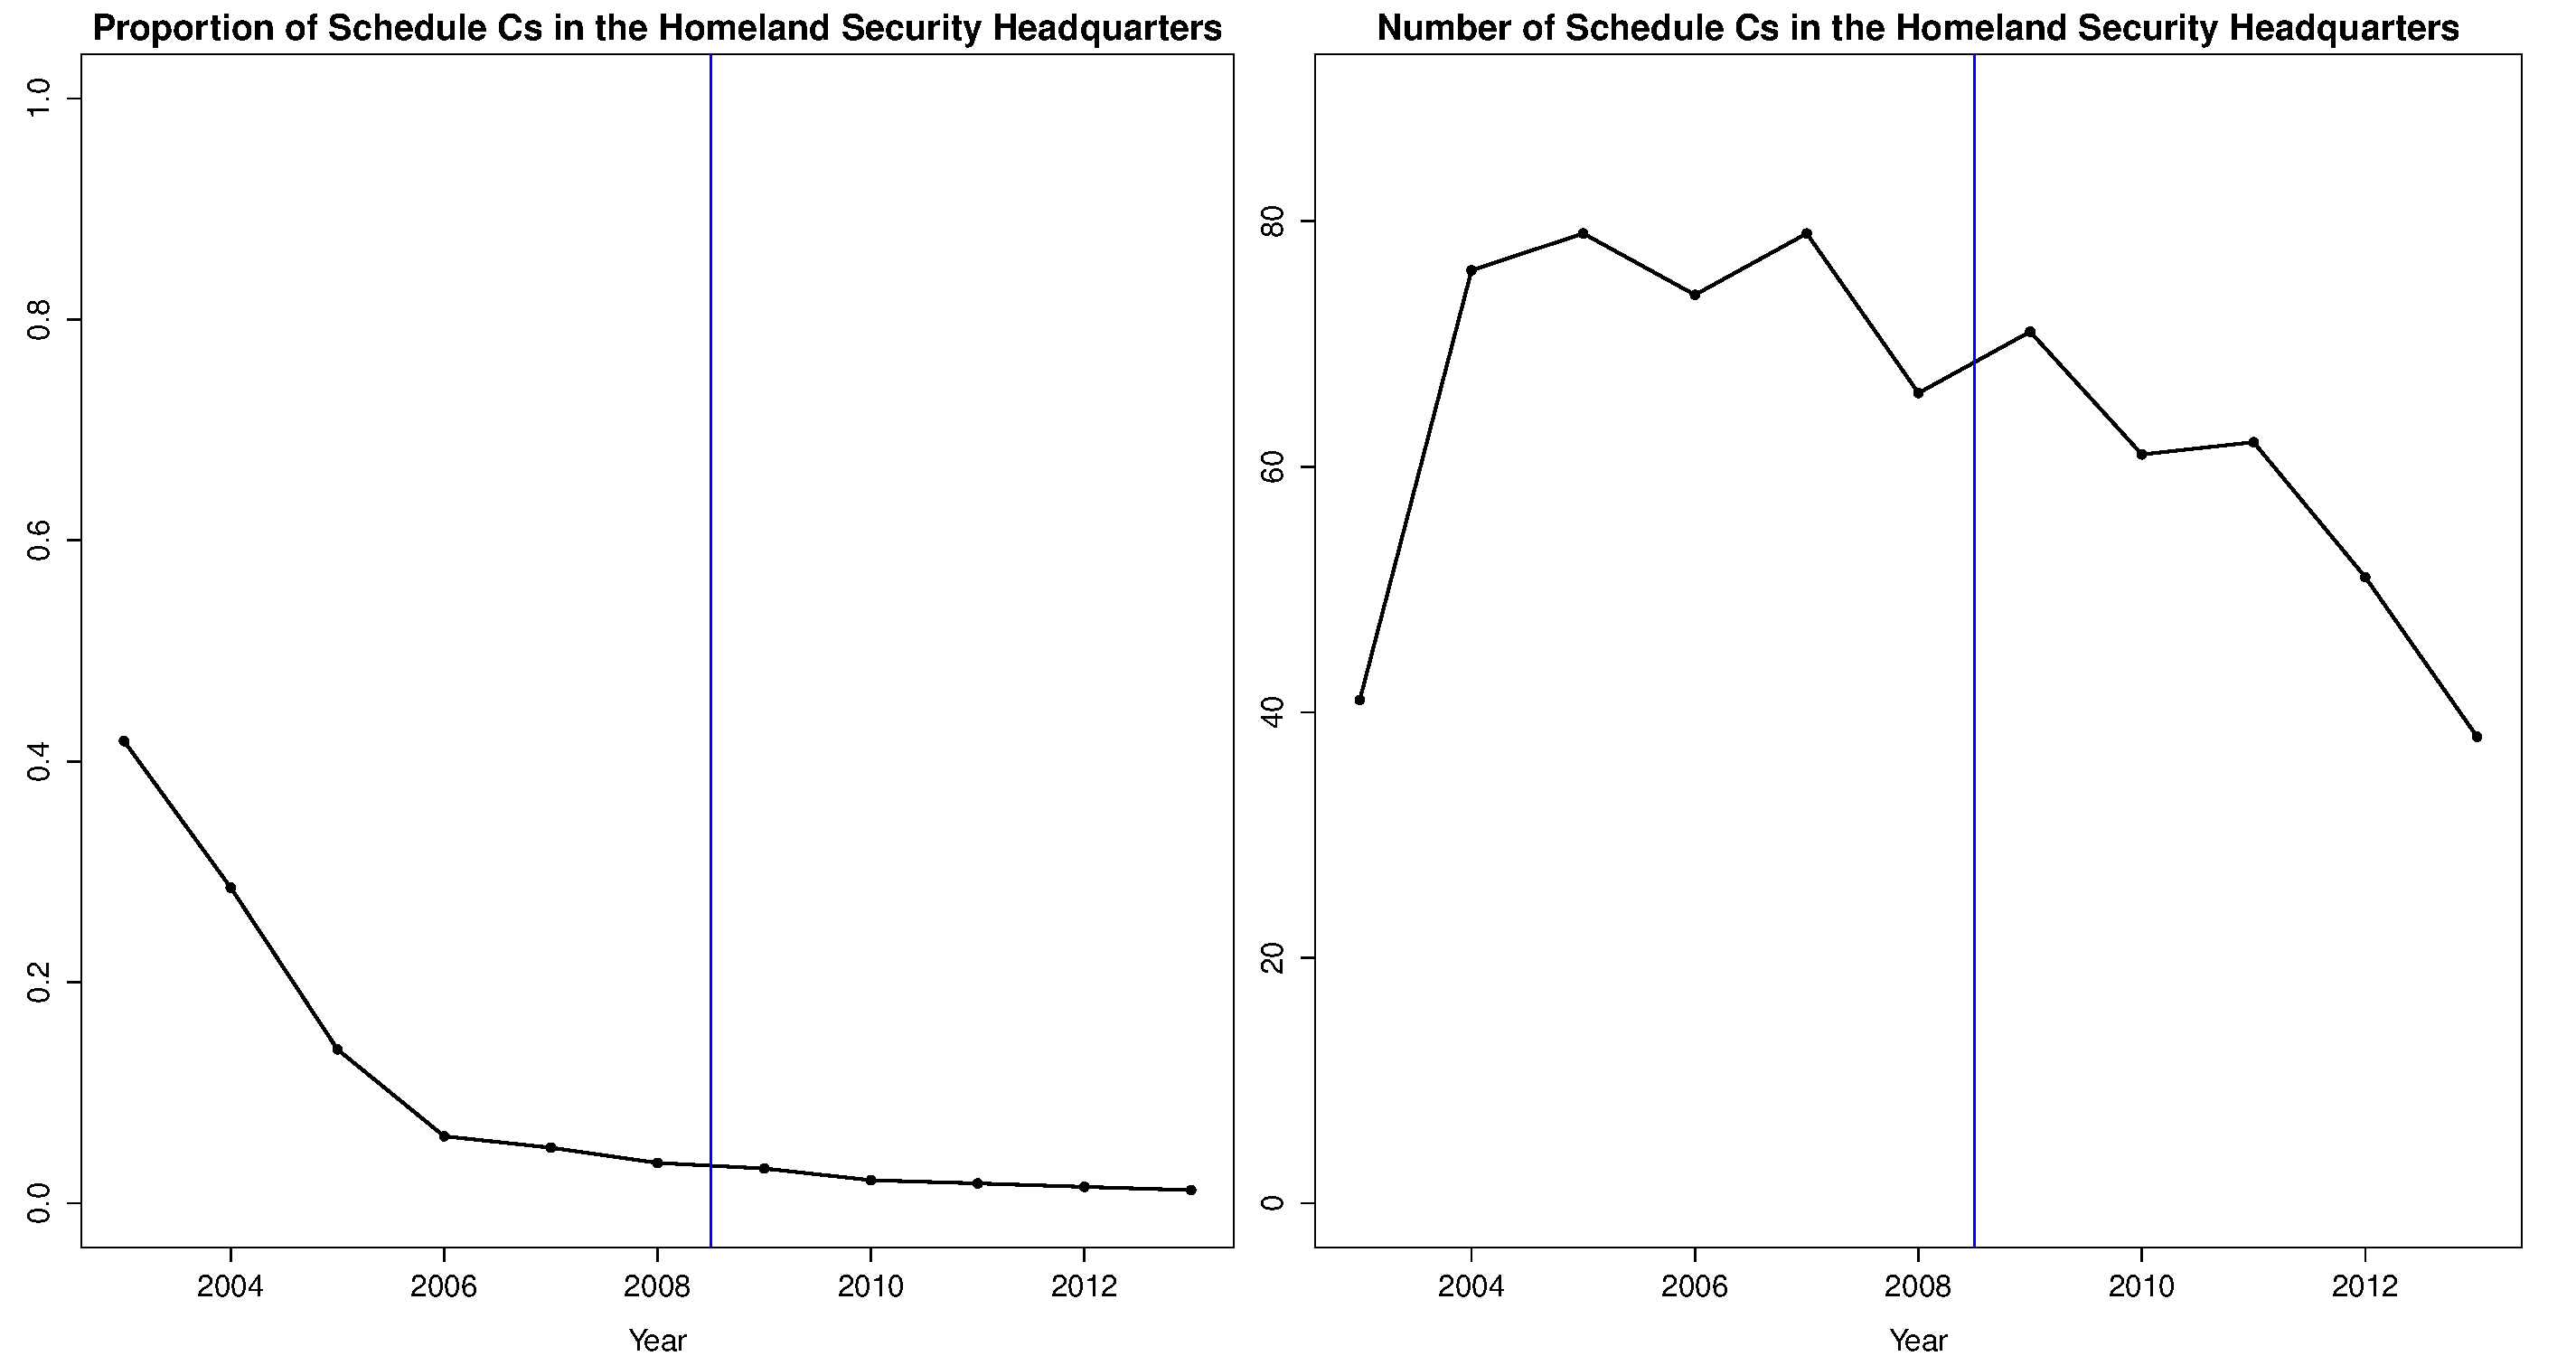
\includegraphics[height=3in,width=6.25in]{DHSProportionRawNumber.pdf}
\caption{Proportion and Raw Number of Schedule C and Excepted Service Executive Appointments in the Homeland Security Headquarters.}
\end{center}
\end{figure}

Figure 2 corroborates the urgency story. In 2003, nearly 50 percent of the Homeland Security Headquarters (OPM has coded it HSAA) was staffed by Schedule C and ESE appointments. This proportion has gradually declined ever since. In the right half of the figure we see the raw number of Schedule C and ESE appointees. The number nearly doubled from 2003 to 2004 yet the proportion of the agency employment made up by Schedule C and ESE appointees declined. This is likely because the president used Schedule C and ESE appointments to fill the department quickly, but as time went on, new hires of other appointment types came in. It is important to note that this declining proportion does not per se indicate declining importance or attention. Rather, it indicates how these appointments can and are used: to act quickly without Congress.


\subsection{Legislative Affairs}

As for the second expectation, we expect to see that liaison agencies, typically public, intergovernmental, or congressional affairs groups should be staffed largely with Schedule C and ESE appointees. 

The left plot of Figure 3 shows the proportion of Department of Labor Congressional Affairs staff that are Schedule C or ESE. Other cabinet agencies and even independent agencies often have congressional or public affairs offices. All of these agencies show similarly above average patterns, but I choose to plot Labor Congressional Affairs. This case is particularly relevant since the Labor Department deals with every congressional district in the United States, which means the Labor Department Congressional Affairs office must deal broadly with members from each district in the country. As can be seen in the plot, the percentage of all employees which were Schedule C or ESE was between about 45 and 75 percent throughout the period. The graph on the right is the average proportion of employees who are Schedule C and ESE across all agencies. This average is usually about 2-3 percent. 

\begin{figure}[h!]
\begin{center}
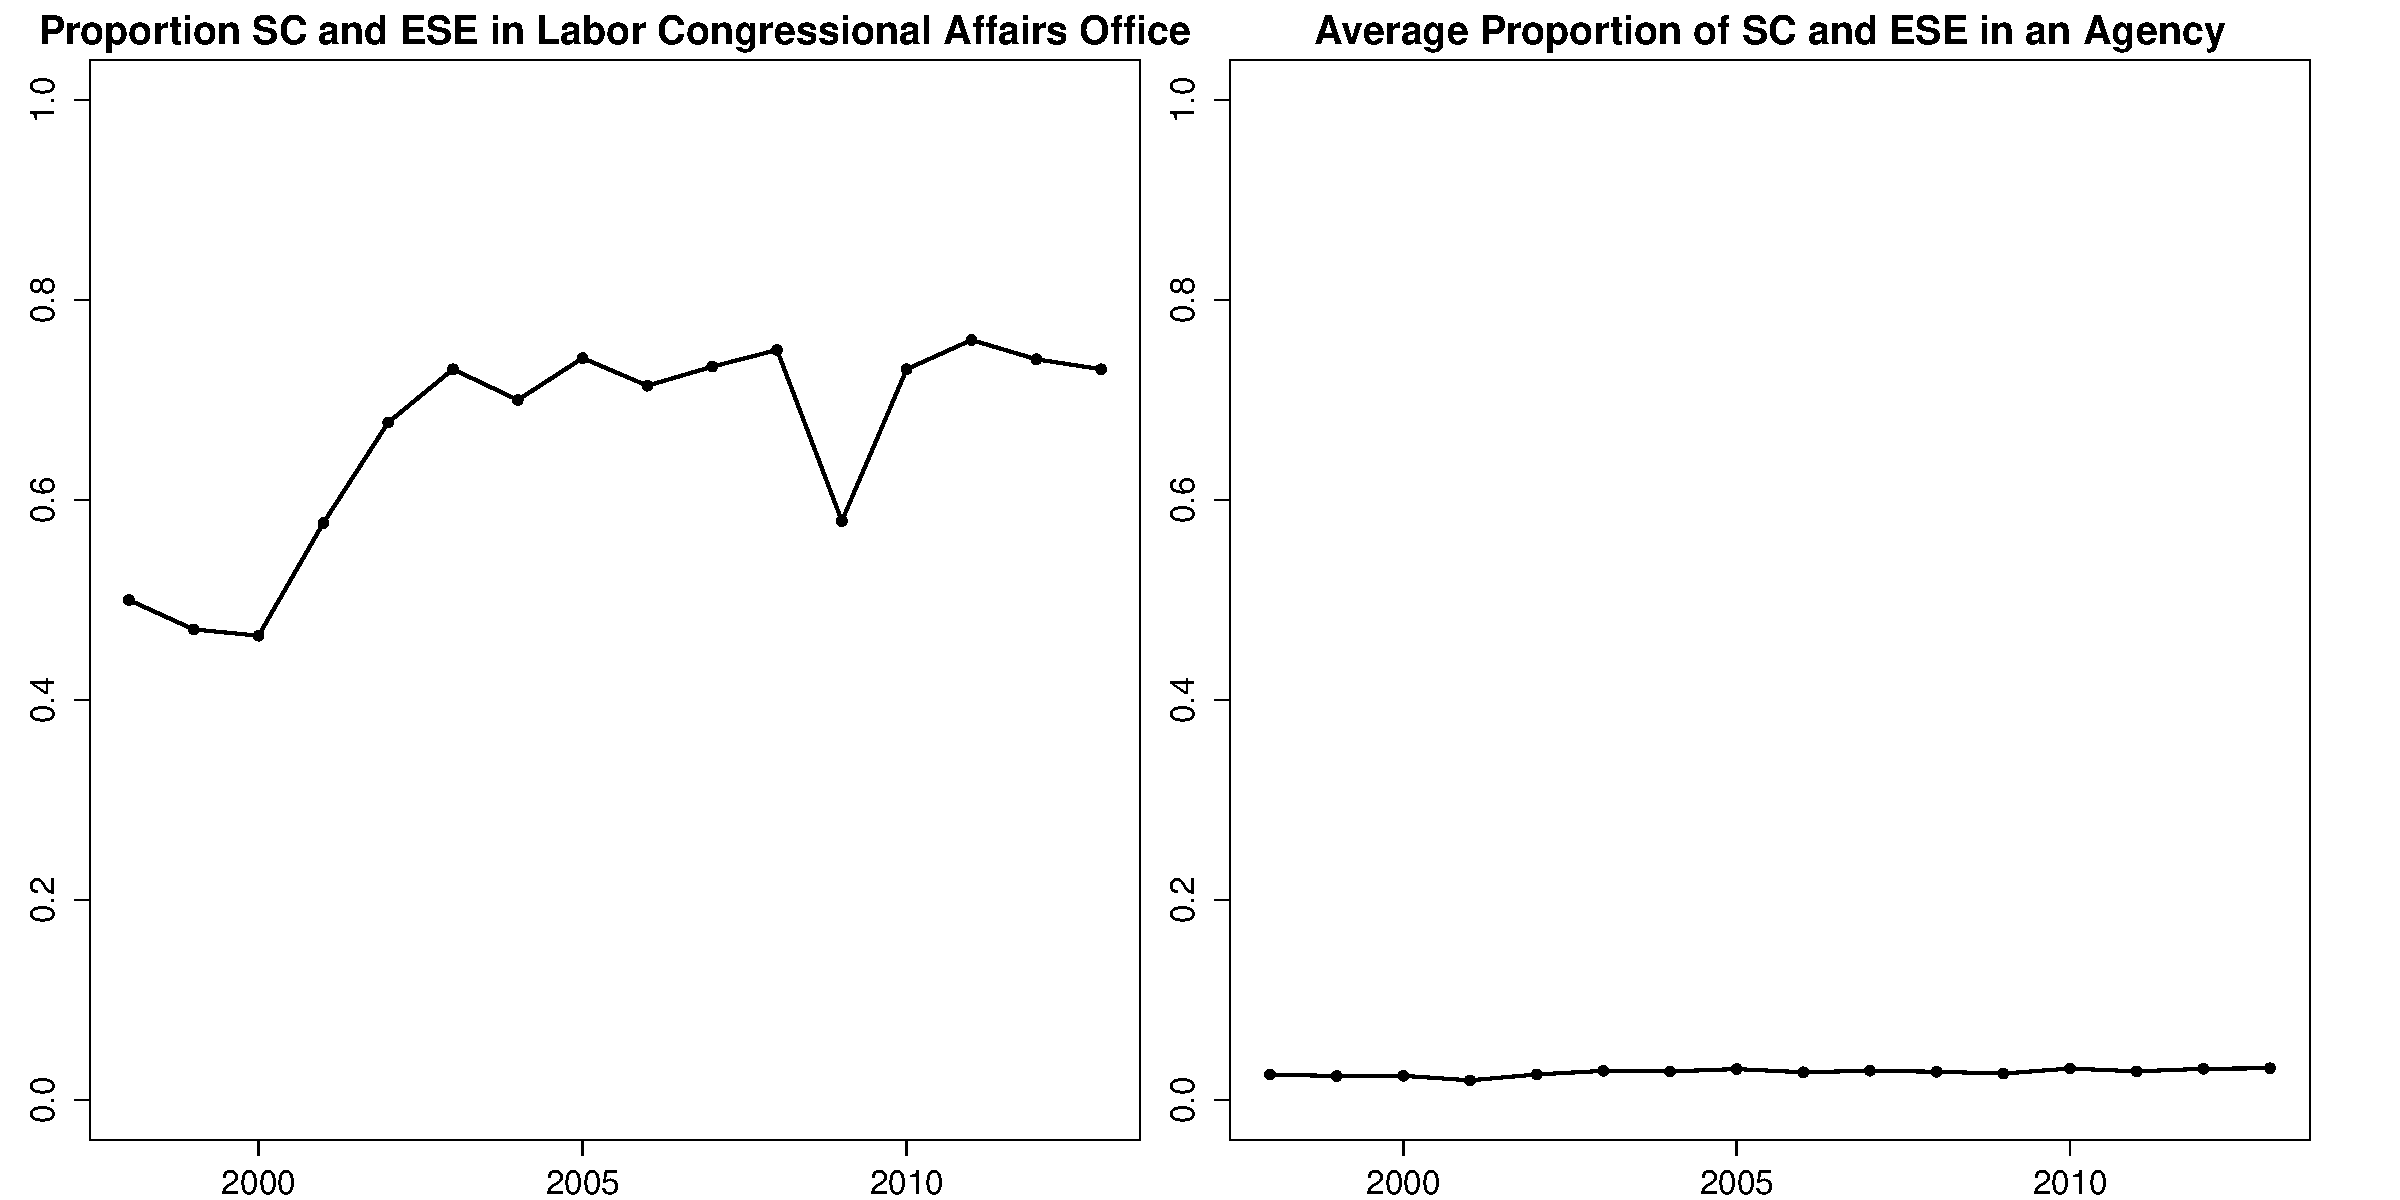
\includegraphics[height=3.5in,width=7in]{LaborCongressionalAffairs.pdf}
\caption{Proportion of Schedule C and Excepted Service Executive Appointments in Labor Congressional Affairs Office as compared to the Average Agency}
\end{center}
\end{figure}

\subsection{Schedule C, ESE, and Ideological Distance from the President}
To test the third expectation from section 4, I ran a negative binomial regression model presdicting counts of Schedule C/ESE appointments using ideological distance of the agency from the president.\footnote{It should be clear that this analysis is not intended as a test of a theory and certainly does not establish a causal relationship. Instead, as with all of these cases, it is meant to serve as a validation of using Schedule C and ESE appointments to study attention. 
}

The ideological distance measure came from two sources. First, I used the agency ideal points calculated by Clinton and Lewis (2008). There are 82 agencies in their data set. This meant reducing the scope of my data from 692 agencies to 78 (because some of the agencies in Clinton/Lewis are not in the Fedscope data). Most of this reduction came in the form of collapsing sub-units into their parent agencies. For example, Clinton/Lewis list all of the cabinet agencies by themselves without sub-organizations. However, some of this reduction also came from eliminating agencies for which Clinton and Lewis do not provide estimates. While Clinton and Lewis do have a wide range of independent agencies of varying size, the Fedscope data is simply more complete. The agency ideal point measure ranges from -2.07 to 2.4 with a mean of 0 and do not vary over time. I then used Poole/Rosenthal estimates for Presidents Clinton, Bush, and Obama to calculate the agency's absolute distance from the president. 

\begin{table}[!htb] \centering 
  \caption{Negative Binomial Regression Results} 
  \label{} 
\begin{tabular}{@{\extracolsep{5pt}}lc} 
\\[-1.8ex]\hline 
\hline \\[-1.8ex] 
 & \multicolumn{1}{c}{\textit{Dependent variable:}} \\ 
\cline{2-2} 
\\[-1.8ex] & SC and ESE Apts \\ 
\hline \\[-1.8ex] 
 Ideology & 0.058 \\ 
  & (0.023) \\ 
  & \\ 
 Bush & 0.007 \\ 
  & (0.023) \\ 
  & \\ 
 Obama & $-$0.018 \\ 
  & (0.025) \\ 
  & \\ 
 Constant & $-$0.011 \\ 
  & (0.506) \\ 
  & \\ 
\hline \\[-1.8ex] 
Observations & 1,213 \\ 
Log Likelihood & $-$3,140.066 \\ 
$\theta$ & 51.100 (6.226) \\ 
Akaike Inf. Crit. & 6,442.132 \\ 
\hline 
\hline \\[-1.8ex] 
\textit{Note: Includes Agency Fixed Effects}  & \\ 
\end{tabular} 
\end{table} 
 
\begin{figure}[htb]
\begin{center}
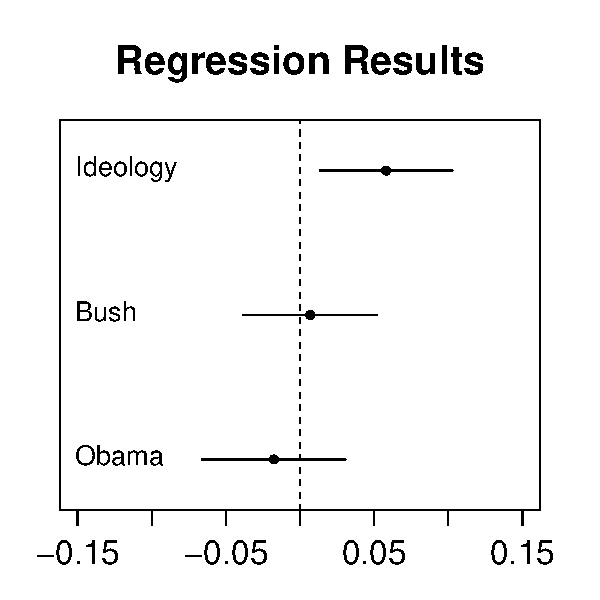
\includegraphics[height=3in,width=3in]{RegressionResults.pdf}
\caption{Negative Binomial Regression Results}
\end{center}
\end{figure}

The outcome variable was simply the number of Schedule C and ESE appointments in an agency in a given year.
 
The results from the negative binomial regression model are shown in Table 1 and visualized in Figure 4. As can be seen, the coefficient for ideological distance is positive and reliable. This means that the president uses more Schedule C and ESE appointments in agencies which are ideologically distant. When the ideological distance increases by 1 (a change from Bush to Obama for a conservative agency), the expected count of SC and ESE appointments is six percent higher.\footnote{This result holds when using the share of attention measure described below in an OLS regression. I also ran the model for each year in the data set individually. The coefficient was consistently positive. While it did not always reach significance, this is likely due to the small sample size (about 70-73 each year). The consistent pattern is reassuring given the time invariant nature of Clinton/Lewis scores.} 

\section{Share of Attention Measurement}
As alluded to before, there are two main qualities of Schedule C and ESE appointments that make them excellent for studying presidential attention. First, Schedule C and ESE appointments are largely ``non-permanent" positions filled only when the president wants them to be.\footnote{There were only 30 permanent ESEs in 2013 of the 2,121 total Schedule C and ESE appointments.} Second, these appointments are flexible and convenient---the president can fill them quickly without the long congressional approval process. As such, we can get an idea of the policy areas or agencies on which the president focuses his human resources at any given time. 

For this purpose, a simple measure of presidential attention is in order. Attention is measured as the share of Schedule C and ESE appointments in a particular agency in a given year over the total number of these appointments in that year. That is, the share of the total number of Schedule C and ESE appointments employed in a given agency is a measure for presidential attention. We can also measure changes in shares of attention over time. In particular, comparisons between presidents in the same year of term (e.g., first year to first year) and within president variation are of interest. Across president comparisons are presented below; within president comparisons are shown in Appendix A.

From a data standpoint, looking at changes in attention is interesting for a few reasons. First, larger agencies in the data automatically draw a larger share of attention from all presidents, so looking at changes in these agencies is more informative. Second, not all agencies report exactly the same. For example, the State Department is artificially inflated relative to the Department of Defense because the State Department reports its employment as a whole whereas DOD reports at the sub-agency and sub-sub-agency level. Thus, the appointments for DOD are spread between dozens of smaller units. 

Each comparison discussed below contains only those agencies which existed in both years to get an accurate comparison of change in attention across or within presidencies. 

\subsection{First Year for Bush and Obama}
One obvious attention comparison is the first years of Bush and Obama. Figure 5 shows the distribution of changes between Obama's share of attention in each agency in 2009 with Bush's share of attention in each agency in 2001. Negative values indicate agencies which received a larger relative share of attention under Bush in his first year than under Obama in his first year. Positive values indicate agencies which received a larger share of attention under Obama's first year. 

There were 410 agencies which existed in both years. Of these, 199 received a value of 0 meaning that attention was the same under Bush and Obama's first years. Some of these agencies are small agencies which did not receive any Schedule C or ESE appointments under either president. Some agencies also receive consistently high levels of attention from both presidents. As discussed above, for example, agencies used in legislative relations have a consistently high proportion of SC and ESE appointees with both presidents and generally do not change much. 

\begin{figure}[htb]
\begin{center}
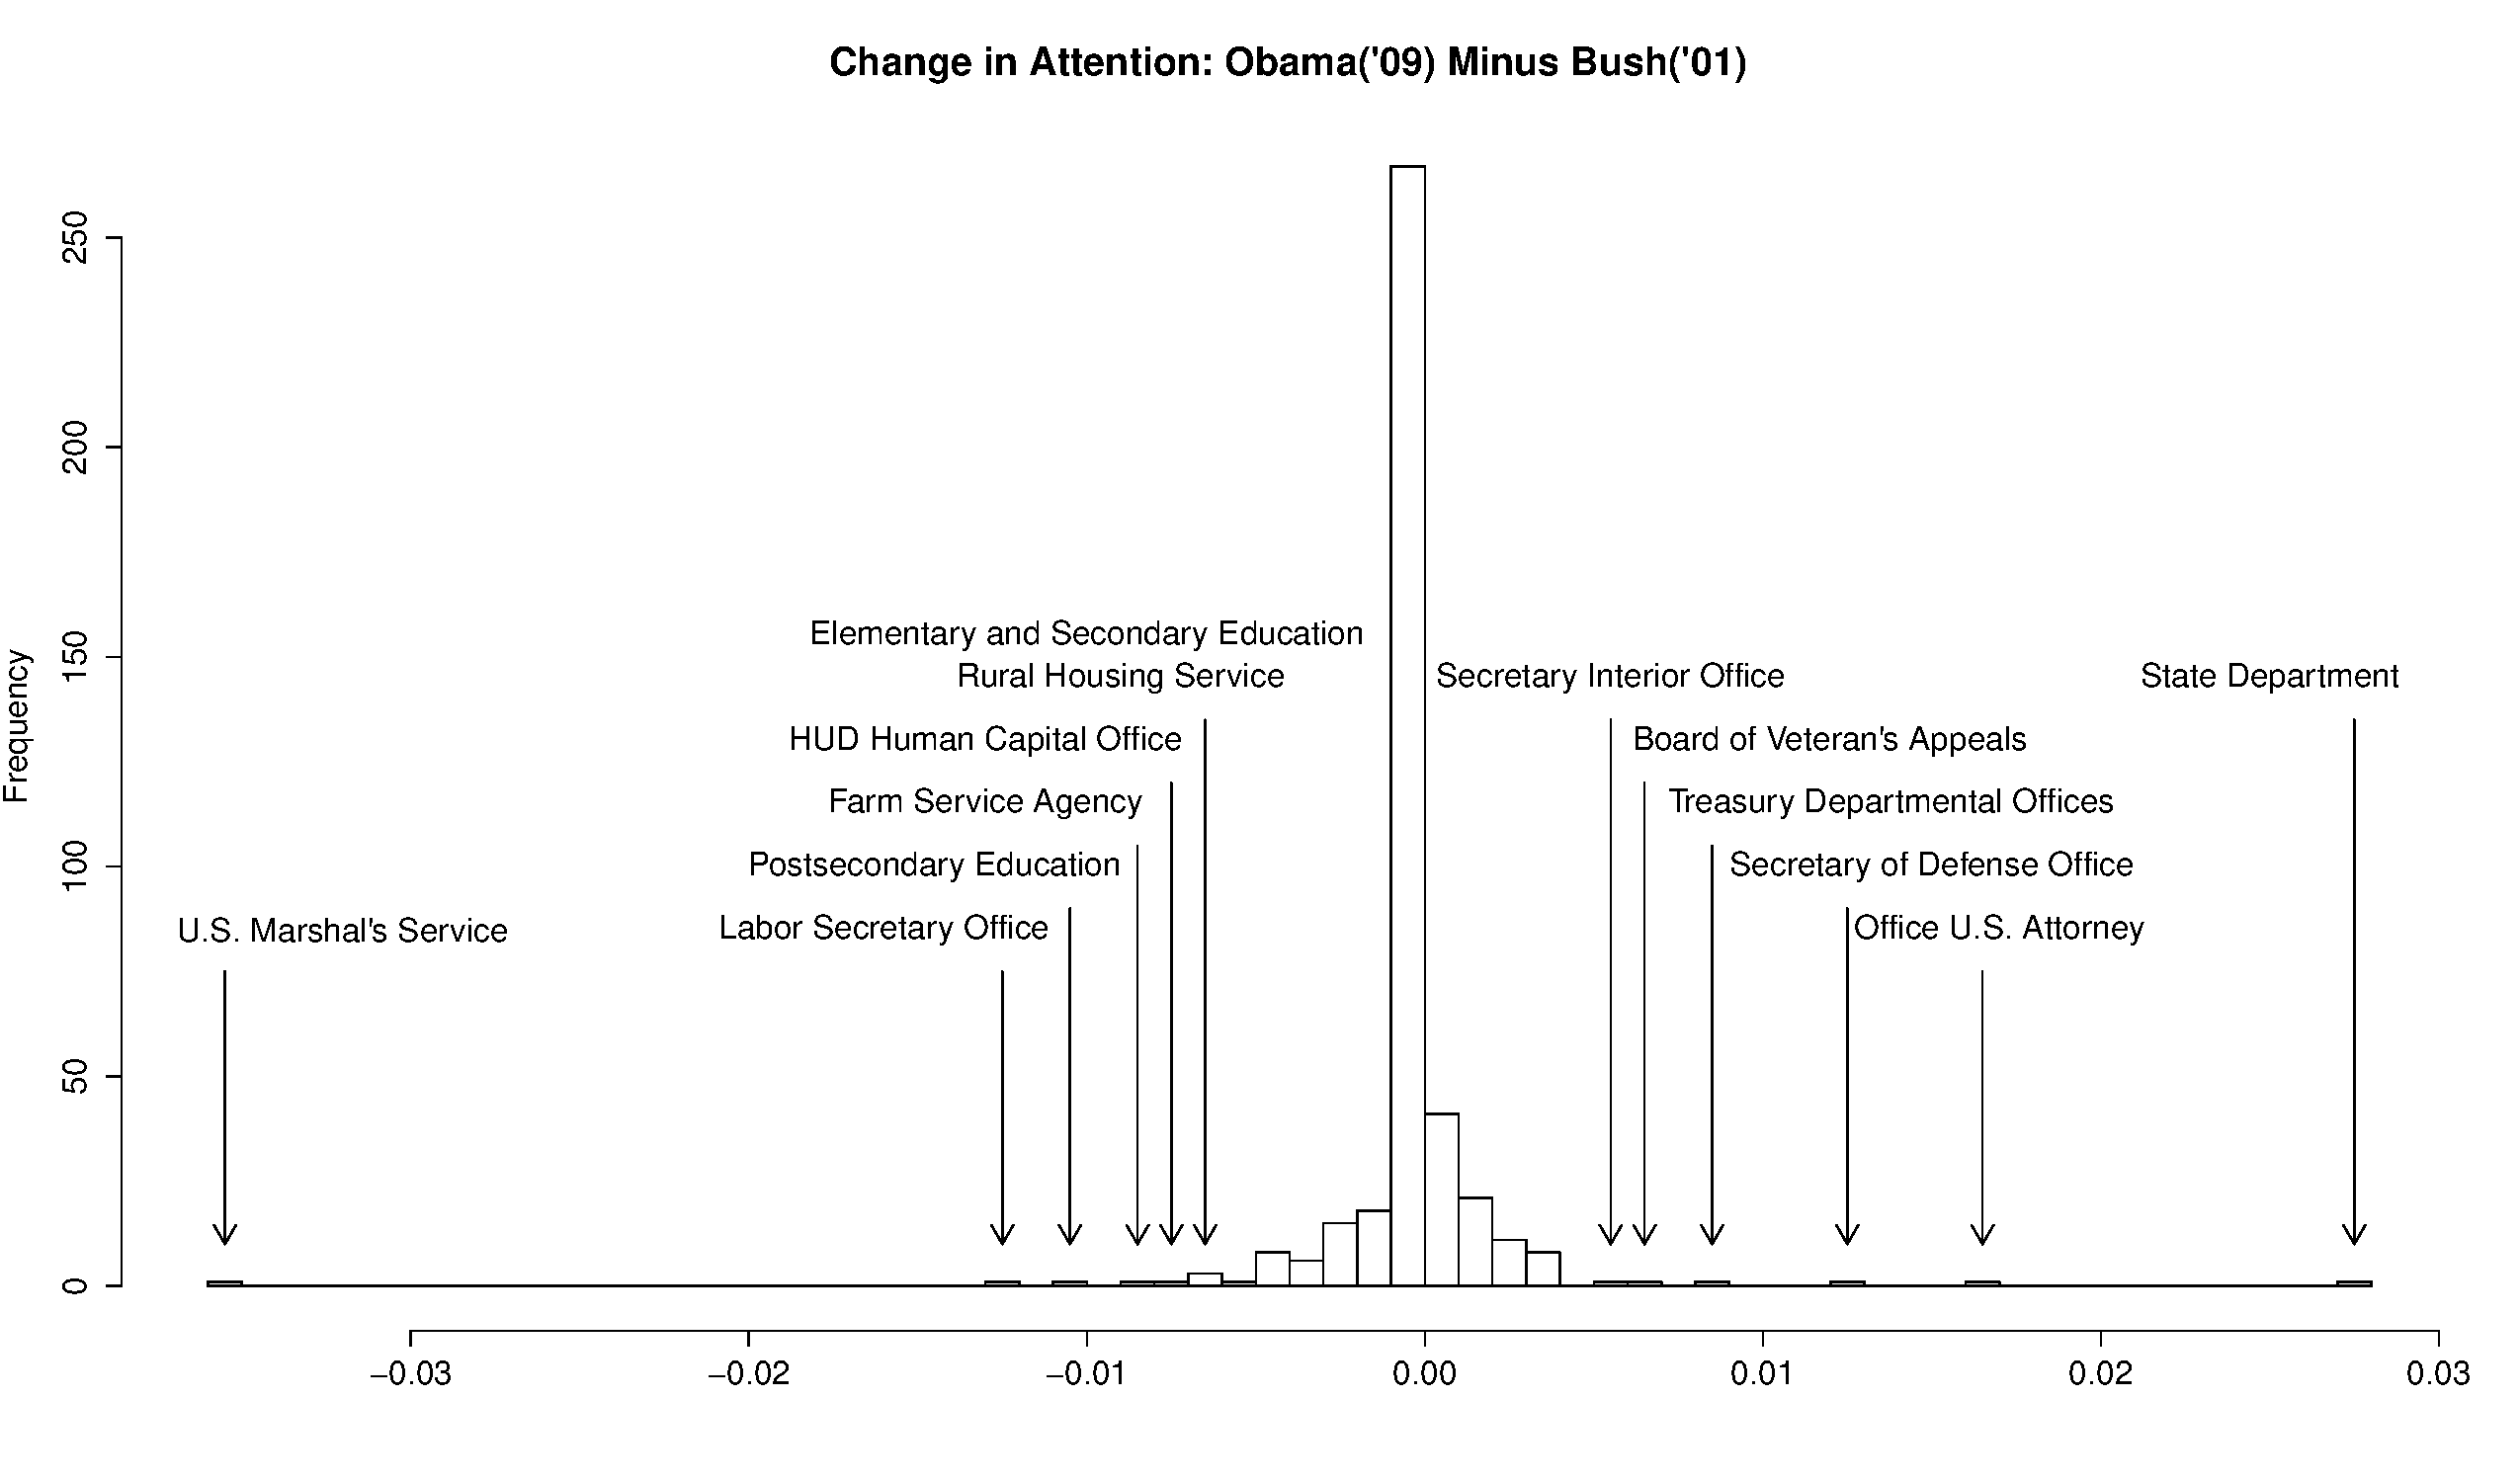
\includegraphics[height=5in,width=7in]{AttentionChange01to09.pdf}
\caption{Changes in Shared Attention between Bush '01 and Obama '09}
\end{center}
\end{figure}

\begin{table}[!htbp] \centering 
\small
  \caption{Top 10 Agencies with Attention Changes 2001 to 2009} 
  \label{} 
\begin{tabular}{@{\extracolsep{5pt}} llllllll} 
\\[-1.8ex]\hline 
More Attention from Bush '01&            &     More Attention from Obama '09&   \\
\hline \\[-1.8ex] 
U.S. Marshal's Service & -0.03501      & State Department         & 0.02721   \\ 
Office of Labor Secretary & -0.01228      & Office U.S. Attorney  & 0.01683    \\ 
Office of Postsecondary Education & -0.01024  & Office Secretary Defense   & 0.01231  \\ 
Farm Service Agency & -0.00804      & Treasury Departmental Offices& 0.00838   \\ 
HUD Human Capital Office & -0.00705   & Board of Veteran's Appeals     & 0.00639   \\ 
Rural Housing Service & -0.00654    & Office Secretary Interior   & 0.00573   \\ 
Elementary and Secondary Education & -0.00630  & Nuclear Waste Technical Review Board&0.00394   \\ 
Office of Justice Programs & -0.00608  & Agriculture Office of Communications  & 0.00394    \\ 
Farm Credit Administration & -0.00502       & Justice Offices, Boards, and Divisions &0.00389  \\ 
Federal Labor Relations Authority & -0.00491    & Office of National Drug Control Policy & 0.00341  \\ 
\hline \\[-1.8ex] 
\end{tabular} 
\end{table} 

Table 2 shows the top ten agencies with more and less attention under Obama than Bush. The left half of the table shows those agencies which received more attention from Bush than Obama (and thus received a negative score), while the right half of the table (like the graph) shows those agencies which received more attention from Obama than Bush. Note the education agencies appearing on the left half, indicating that Bush spent more attention on these agencies in his first year than Obama did in his. This attention difference is sensible given the passage of No Child Left Behind in 2001. Obama's greater focus on the Nuclear Waste Technical Review Board in 2009 may be a function of nuclear arms treaty negotiations with Russia for the New START treaty that year, although it is difficult to be certain. 

\subsection{Second Year for Bush and Obama}

\begin{figure}[htb]
\begin{center}
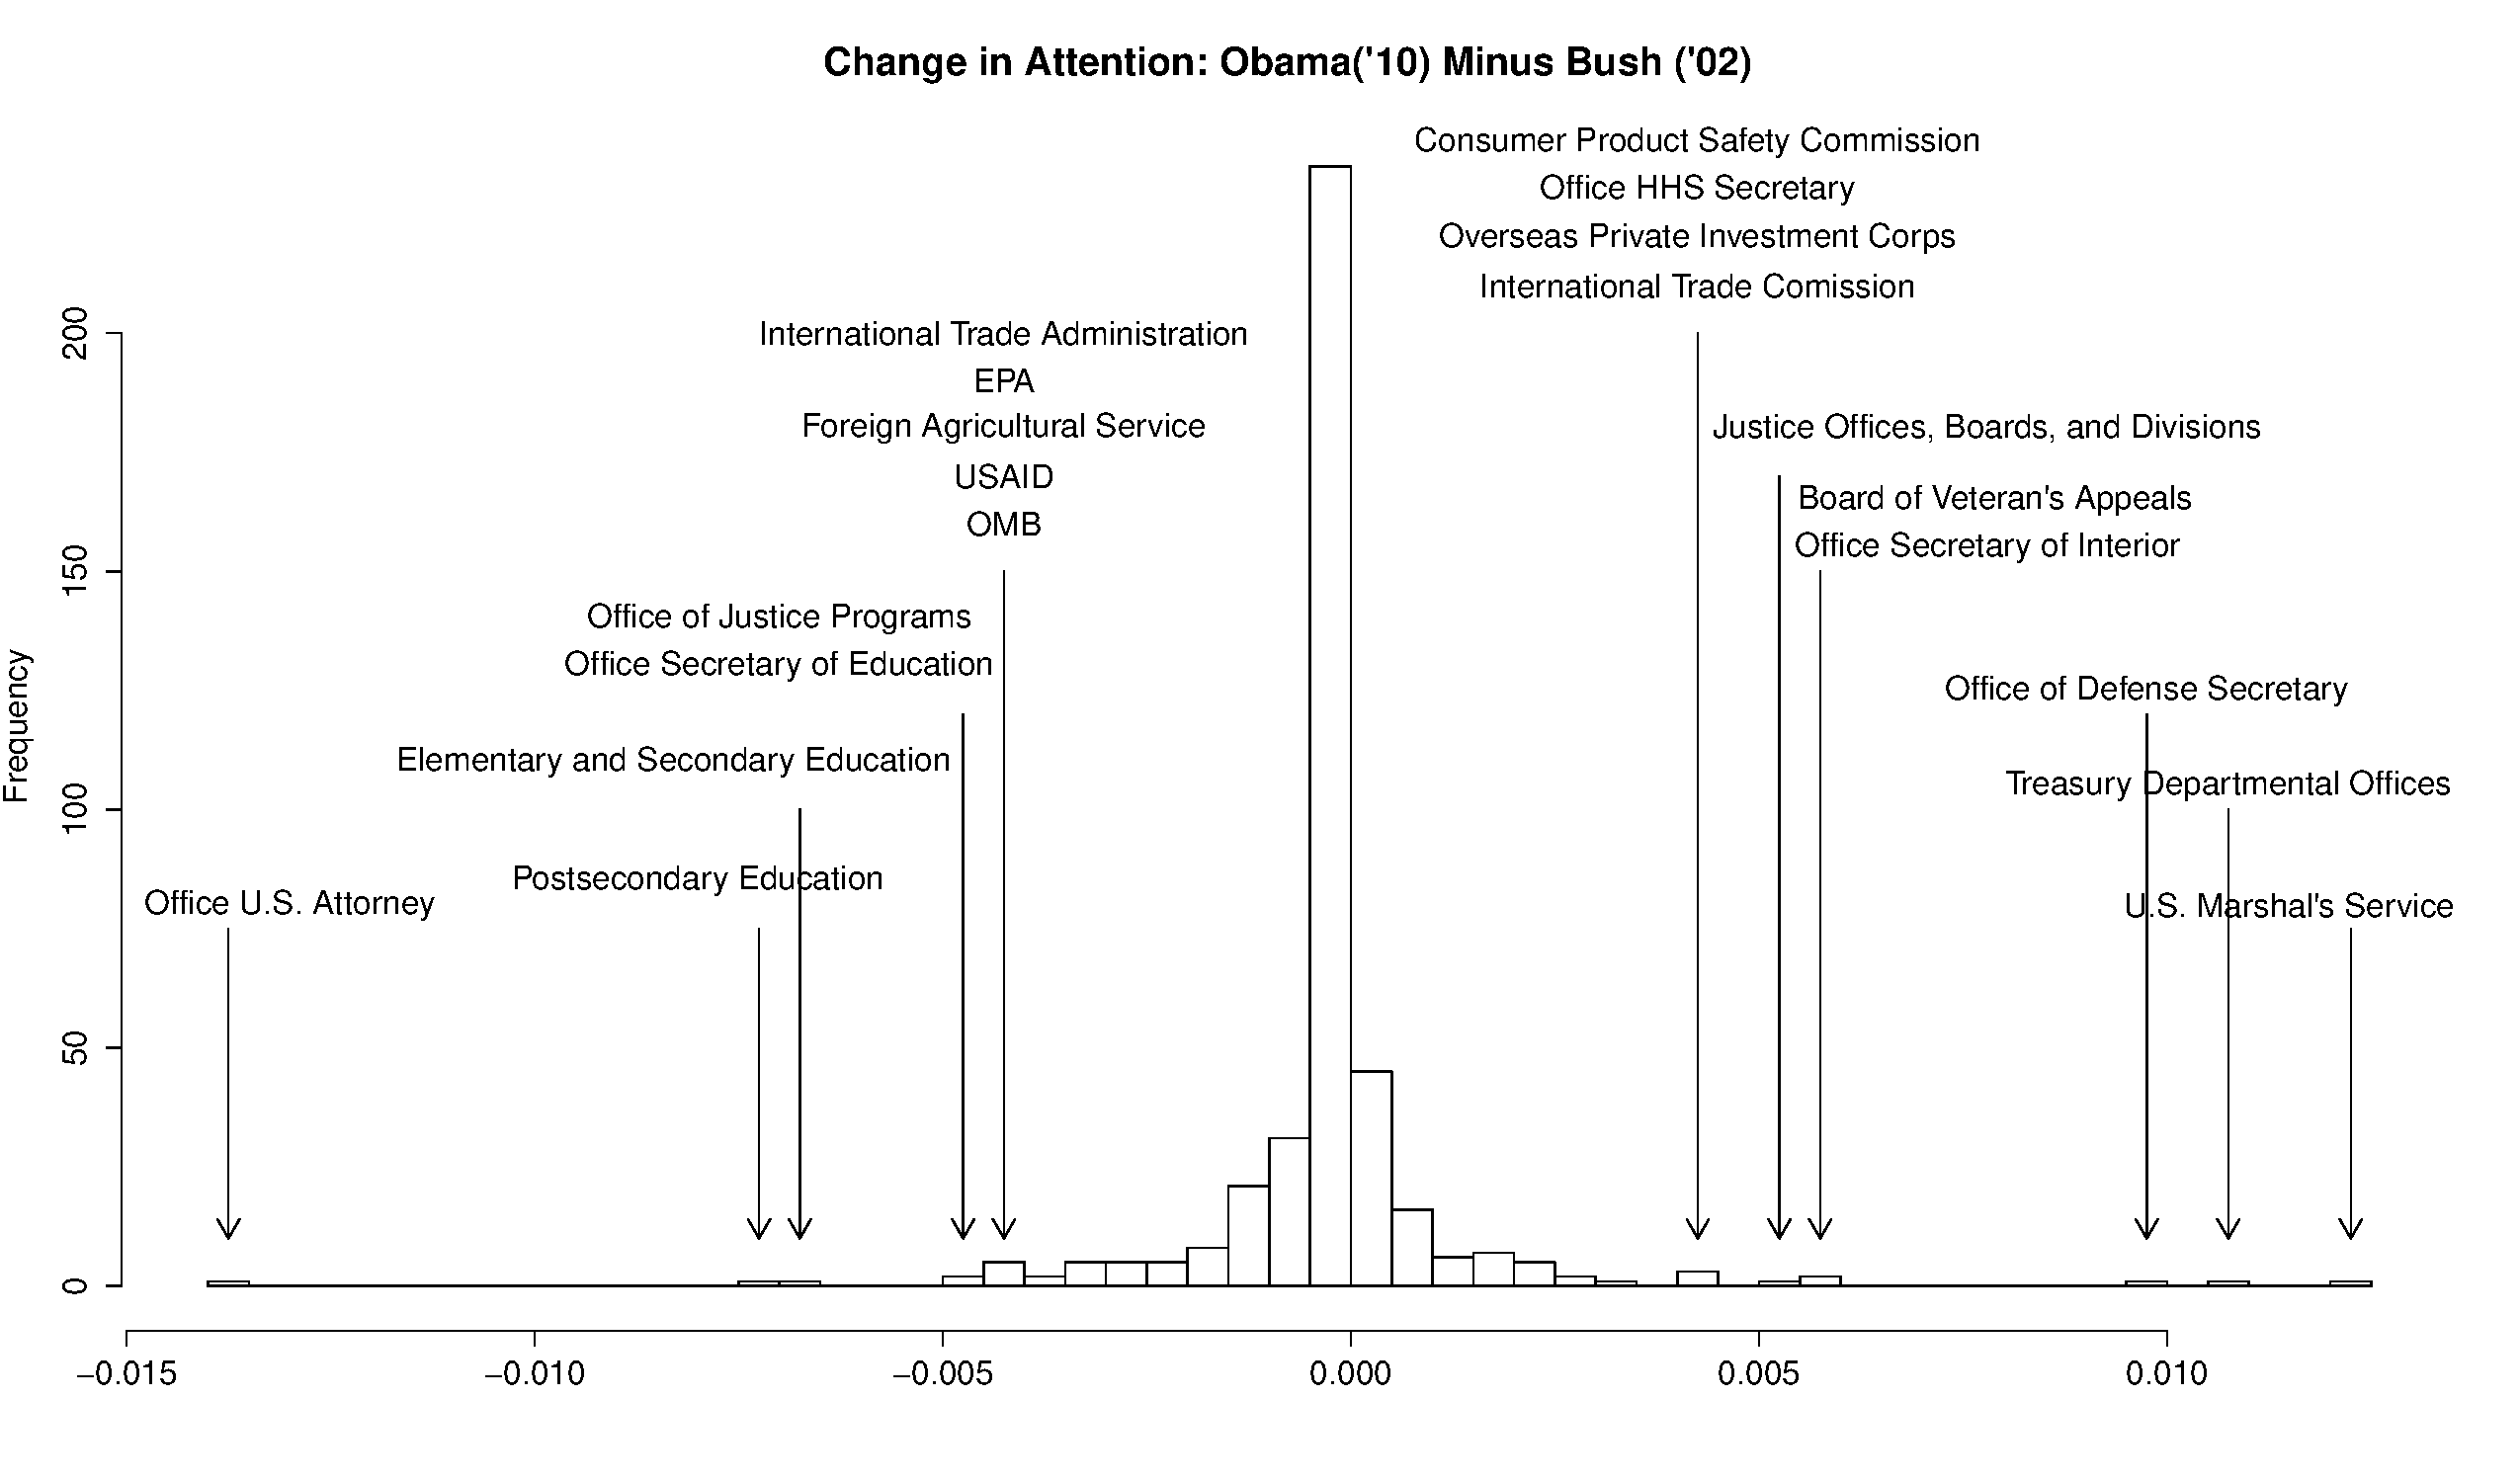
\includegraphics[height=5in,width=7in]{AttentionChange02to10.pdf}
\caption{Changes in Shared Attention between Bush '02 and Obama '10}
\end{center}
\end{figure}

\begin{table}[!htbp] \centering 
\small
  \caption{Changes in Shared Attention Between Bush 2002 and Obama 2010} 
  \label{} 
\begin{tabular}{@{\extracolsep{5pt}} lllllll} 
\\[-1.8ex]\hline 
More Attention Under Bush '02 &&More Attention Under Obama '10 & \\
\hline \\[-1.8ex] 
Office U.S. Attorney & -0.01390 & U.S. Marshal's Service & 0.01240 \\ 
Office Postsecondary Education & -0.00720 & Treasury Departmental Offices &0.01054 \\ 
Elementary and Secondary Education & -0.00693 & Office Defense Secretary&0.00958 \\ 
Office of Justice Programs & -0.00498 & Office Secretary Interior & 0.00595 \\ 
Office of Secondary Education & -0.00460 & Board Veterans Appeals & 0.00567 \\ 
OMB & -0.00448 & Justice Offices, Boards, and Divisions&0.00519 \\ 
USAID & -0.00437 & Consumer Product Safety Commission & 0.00446 \\ 
Foreign Agricultural Service & -0.00434 & Office Secretary HHS & 0.00446 \\ 
EPA & -0.00416&Overseas Private Investment Corp. & 0.00426 \\ 
International Trade Administration & -0.00408 & International Trade Commission & 0.00341 \\ 
\hline \\[-1.8ex] 
\end{tabular} 
\end{table} 

The second year comparison may be more valuable than the first year comparison for Bush and Obama. This is because the comparison will be on a strictly post-9/11 basis and also because accessions continue to be inflated in the first few months of the second year of office. Figure 6 shows this comparison. There were 413 agencies which existed in both years. Of these, 178 had no change. 

As is visible from the figure and Table 3, some agencies which had been listed under Bush or Obama in the first year comparison have reversed. It may be a simple difference in timing. For example, while the Office of the U.S. Attorney (DJO9) received more attention in Obama's first year than Bush's, it received more attention from Bush's second year than Obama's. Likewise, the U.S. Marshal's Service (DJ08) received more attention in Bush's first year and Obama's second year. This likely indidicates that these offices are important to both presidents, but they prioritized them differently. 

Education is still of higher attention in Bush's second year than Obama's. Interestingly, in 2010, we see that Obama has increased attention (relative to Bush) in Health and Human Services, which makes a great deal of sense given the passage of the Affordable Care Act that year. 

Bush's focus on USAID is likely a function of the War on Terror. In the 2002 \textit{Accountability Report Transmittal Letter}, USAID Administrator Andrew Natsios wrote that USAID had a ``challenging year" as they ``faced the consequences of the war on terrorism." He further argues that President Bush ``raised the strategic importance of development to the point that it is now an essential pillar of U.S. foreign policy alongside defense and diplomacy" (USAID 2002, pg 3.) The report emphasizes new goals and sets of duties set forth by the President in that year, so it should come as no surprise that USAID received more attention from Bush in 2002 than Obama in 2010. The report further emphasizes Bush's desire that USAID engage in trade programming. In that light, his focus on the International Trade Commission is also telling. Finally, the USAID report also mentions its work with the USDA providing relief in Africa and Afghanistan, suggesting Bush's relative emphasis on the Foreign Agricultural Service as well. 

\section{Conclusion}

As this paper has hopefully demonstrated, presidential attention is an important but understudied concept. While scholars have examined how presidents choose bureaucrats, we know little about how they apportion more flexible personnel. I have found that presidents use these appointments in ways we would expect. First, presidents use flexible personnel to staff agencies quickly when the situation is urgent. Second, presidents staff agencies tasked with communicating the administration's message to Congress and the public with flexible, political appointees. Presidents also focus more appointments in ideologically dissimilar agencies than they do in like-minded ones. Perhaps this is because the president expects to have more trouble pursuing his agenda when it is at odds with the agency's predisposition.

In addition to how presidents generally use lower level appointees, they also differ in how they distribute attention. While some agencies receive a consistent portion of agency attention, others receive more attention if that issue is on the president's agenda. For example, subagencies within the Department of Education received more attention from President Bush as he pushed for No Child Left Behind and Health and Human Services received more attention during Obama's fight for the Affordable Care Act. These findings only begin to paint a picture of presidential attention, but will hopefully provide a basis for considering its implications for bureaucratic politics in the future. 

\section{References}
\noindent \hangindent=0.7cm Aberbach, Joel D.,  and Bert A. Rockman. 1976. ``Clashing Beliefs withing the Executive Branch: The Nixon Administration Bureaucracy." \textit{American Political Science Review} 70(2): 456-468. 

\noindent \hangindent=0.7cm Aberbach, Joel D., and Bert A. Rockman. 1995. ``The Political Views of U.S. Senior Federal Executives, 1970-1992. \textit{Journal of Politics} 57(3): 838-52. 

\noindent \hangindent=0.7cm Aberbach, Joel D., and Bert A. Rockman. 2000. \textit{In the Web of Politics: Three Decades of the U.S. Federal Executive.} Washington, DC: Brookings.

\noindent \hangindent=0.7cm Bertelli, Anthony and Christian Grose. 2009. ``Secretaries or Pork? A New Theory of Distributive Poltics." \textit{Journal of Politics} 71(3): 926-945. 

\noindent \hangindent=0.7cm Barr, Stephen. 2008. ``DHS Withdraws Bid to Curb Union Rights." \textit{Washington Post}. \url{http://www.washingtonpost.com/wp-dyn/content/article/2008/02/1/AR2008021902459.html}. Last accessed January 6, 2014.

\noindent \hangindent=0.7cm Burke, John P. 1992. \textit{The Institutional Presidency}. Baltimore: Johns Hopkins University Press. 

\noindent \hangindent=0.7cm Clinton, Joshua D., Anthony Bertelli, Christian Grose, David E. Lewis and David C. Nixon. 2012. ``Separated Powers in the United States." American Journal of Political Science, 56(2):341-54.

\noindent \hangindent=0.7cm Clinton, Joshua D., and David E. Lewis. 2008. "Expert Opinion, Agency Characteristics, and Agency Preferences." Political Analysis 16:3-20.

\noindent \hangindent=0.7cm Cohen, David M. 1988. ``Amateur Government." \textit{Journal of Public Administration Research and Theory} 8(4):450-97. 

\noindent \hangindent=0.7cm Cohen, Jeffery E. 1995. ``Presidential Rhetoric and the Public Agenda." \textit{American Journal of Political Science} 39:87-107. 

\noindent \hangindent=0.7cm Edwards III, George C. and B. Dan Wood. 1999.``Who Influences Whom? The President, Congress, and the Media." \textit{American Political Science Review} 93(2): 327-344.

\noindent \hangindent=0.7cm Epstein, David, and Sharyn O'Halloran. 1999. \textit{Delegating Powers}. New York: Cambridge University Press. 

\noindent \hangindent=0.7cm Fenno, Richard F. 1959. \textit{The President's Cabinet: An Analysis in the Period from Wilson to Eisenhower.} Cambridge, MA: Harvard University Press.

\noindent \hangindent=0.7cm Gailmard, Sean and John W. Patty. 2012. \textit{Learning While Governing.} Chicago: University of Chicago Press. 

\noindent \hangindent=0.7cm Gilmour, John B., and David E. Lewis. 2006. ``Political Appointees and the Competence of Federal Program Management." \textit{American Politics Research} 34(1):22-50. 

\noindent \hangindent=0.7cm Harrabin, Roger. 2006.  ``Mixed Outcomes at Climate Talks." \textit{BBC}. \url{http://news.bbc.co.uk/2/hi/science/nature/5408798.stm.} Last accessed January 6, 2014.

\noindent \hangindent=0.7cm Hart, John. 1995. \textit{The Presidential Branch}.  New York: Chatham House.

\noindent \hangindent=0.7cm Heclo. 1975. ``OMB and the presidency---The problem of `neutral competence.'" \textit{Public Interest} 38(Winter): 80-98.

\noindent \hangindent=0.7cm Heclo. 1977. \textit{A Government of Strangers: Executive Politics in Washington}. Washington, DC: Brookings Institution.

\noindent \hangindent=0.7cm Hill, Kim Quaile. 1998. ``The Policy Agendas of the President and the Mass Public: A Research Validation and Extension." \textit{American Journal of Political Science}42(4): 1328-1334.

\noindent \hangindent=0.7cm Hollibaugh, Gary E. forthcoming. "Na�ve Cronyism and Neutral Competence: Patronage, Performance, and Policy Agreement in Executive Appointments" \textit{Journal of Public Administration Research and Theory}. 

\noindent \hangindent=0.7cm Hollibaugh Jr., Gary E., Gabe Horton, and David E. Lewis. Forthcoming. ``Presidents and Patronage." \textit{American Journal of Political Science.}

\noindent \hangindent=0.7cm Lewis, David E. 2003. \textit{Presidents and the Politics of Agency Design: Political Insulation in the United States Government Bureaucracy, 1946-1997.} Stanford, CA: Stanford University Press.

\noindent \hangindent=0.7cm Lewis, David E. 2005. ``Staffing Alone: Unilateral Action and the Politicization of the Executive Office of the President, 1988-2004." \textit{Presidential Studies Quarterly} 35(3): 496-514.

\noindent \hangindent=0.7cm Lewis, David E. 2008.\textit{The Politics of Presidential Appointments: Political Control and Bureaucratic Performance}. Princeton, NJ: Princeton University Press. 

\noindent \hangindent=0.7cm Lewis, David, E and Richard W. Waterman. 2013. ``The Inivisible Presidential Appointments: An Examination of Appointments to the Department of Labor, 2001-11.'' \textit{Presidential Studies Quarterly} 43(1): 35-57.

\noindent \hangindent=0.7cm Mackenzie, G. Calvin. 1981. \textit{The Politics of Presidential Appointments}. New York: Free Press. 

\noindent \hangindent=0.7cm Mann, Dean E. 1964. ``The Selection of Federal Political Executives." \textit{American Political Science Review} 58(1): 81-99. 

\noindent \hangindent=0.7cm McCubbins, Mathew D. and Thomas Schwartz. 1984. ``Congressional oversight overlooked: Police patrols versus fire alarms." \textit{American Journal of Political Science} 28: 16-79. 

\noindent \hangindent=0.7cm McKeown, Timothy. 2005. ```Micromanagement' of the U.S. Aid Budget and the Presidential Allocation of Attention." \textit{Presidential Studies Quarterly} 35(2): 319-332.

\noindent \hangindent=0.7cm  Moe, Terry M. 1985. ``The Politicized Presidency." In \textit{The New Direcion in American Politics}, edited by J. E. Chubb and P.E. Peterson. Washington, DC. Brookings Institution. 

\noindent \hangindent=0.7cm National Environmental Policy Act. 1969. \textit{U.S. Statutes at Large} 83 (1970): 852.

\noindent \hangindent=0.7cm Parsneau, Kevin. 2013. ``Politicizing Priority Departments: Presidential Priorities and Subcabinet Experience and Loyalty." \textit{American Politics Research} 41(3):443-70.

\noindent \hangindent=0.7cm Patterson, Bradley H. 2008. \textit{To Serve the President: Continuity and Innovation in the White House Staff.} Washington, DC: Brookings Institution Press.

\noindent \hangindent=0.7cm Patterson, Bradley H. and James P. Pfiffner. 2001. ``The White House Office of Presidential Personnel." \textit{Presidential Studies Quarterly} 31(3):415-438.

\noindent \hangindent=0.7cm Pfiffner, James P. 2015. ``Presidential Appointments and Managing the Executive Branch." Political Appointee Project. \url{http://www.politicalappointeeproject.org/commentary/appointments-and-managing-executive-branch} (April 9, 2015).

\noindent \hangindent=0.7cm Revkin, Andrew. 2005a. ``Bush Aide Softened Greenhouse Gas Links to Global Warming." \textit{New York Times}. \url{http://www.nytimes.com/2005/06/08/politic/08climate.html?ei=5090 &en=22149dc70c0731d8&ex=1275883200&partner=rssuserland&emc=rss.}Last Accessed January 6, 2015.

\noindent \hangindent=0.7cm Revkin, Andrew. 2005b. ``Editor of Climate Reports Resigns." \textit{New York Times}. \url{http://www.nytimes.com/2005/06/10/politics/11cooney.long.html?ex =1276056000&en=7da9d69d3b1ecb1a&ei=5090&partner=rssuserland&emc=rss&_r=0.} Last Accessed January 6, 2015. 

\noindent \hangindent=0.7cm Tolchin, Martin, and Susan Tolchin. 2010. \textit{Pinstripe Patronage: Political Favoritism from the Clubhouse to the White House and Beyond.} Boulder, CO: Paradigm Publishers.

\noindent \hangindent=0.7cm United States Agency for International Development. 2002. \textit{Performance and Accountability Report.}Washington: United States Agency for International Development.

\noindent \hangindent=0.7cm United States House of Representatives. Committee on Oversight and Government Reform. 2012. 112th 2nd. \textit{Policy and Supporting Positions}(Plum Book). 

\noindent \hangindent=0.7cm Wayne, Stephen J., Richard L. Cole, and James F.C. Hyde, Jr. 1979. ``Advising the President on Enrolled Legislation: Patterns of Executive Influence." \textit{Political Science Quarterly} 94(2): 303-16. 

\noindent \hangindent=0.7cm Wood, B. Dan and Richard W. Waterman. 1994. \textit{Bureaucratic Dynamics: The Role of Bureaucracy in a Democracy, Transforming American Politics}. Boulder: Westview Press. 


\section{Appendix A: Within Presidency Attention Changes}
\subsection{Bush Unified Government and Divided Government}

\begin{table}[!htbp] \centering 
\small
  \caption{Attention changes Bush in 2006 and 2007} 
  \label{} 
\begin{tabular}{@{\extracolsep{5pt}} lllllll} 
\\[-1.8ex]\hline 
More Attention in 2006 &&More Attention in 2007 & \\
\hline \\[-1.8ex] 
Office U.S. Attorney & -0.00641          & Department of Energy &  0.00414 \\ 
Just. Ofs, Boards, and Divs. & -0.00465& Ofc. Secretary Defense& 0.00374 \\ 
Nuclear Detection Office& -0.00434     & Natl Science Found.& 0.00371 \\ 
Defense Commissary Agency & -0.00257   & U.S. Intl Trade Comm. & 0.00286 \\ 
Ofc. of Justice Programs & -0.00219    & Treas. Departmental Ofcs. & 0.00261 \\ 
NOAA &  -0.00217                       & Inst. Museum and Library Serv.& 0.00244 \\ 
Naval Medical Command & -0.00173       & Small Business Admin. & 0.00234 \\ 
Broadcasting Board of Govs. & -0.00172 & Board Veteran's Appeals& 0.0021 \\ 
Office Sec. Commerce &  -0.00153       & Natl Endowment Arts & 0.00202 \\ 
EPA & -0.00153                         & Rural Housing & 0.00186 \\ 
\hline \\[-1.8ex] 
\end{tabular} 
\end{table} 

Table 4 shows the comparison between Bush in '06 with his last year of unified government and Bush in '07 under the first year of divided government. Of the 519 agencies, 257 did not have an attention change between 2006 and 2007. Of course, it is important to note that the numbers represent changes in attention. Agencies may receive consistently high attention from Bush over the period and receive a score of 0. Rather, the values are important because they represent how Bush's attention changed over the period. 

Agencies which received more attention in unified government under Bush can be seen in the left of Table 4. The Homeland Security Domestic Nuclear Detection Office received more attenion in 2006. As did the Defense Commissary Agency, the National Oceanic and Atmospheric Administration, the EPA, the Naval Medical Command, the Broadcasting Board of Governors, and the Secretary of Commerce's office. 

When the Democratic Congress took office, Bush's attention shifted in favor of the Department of Energy, Defense Secretary's Office, the National Science Foundation, the U.S. International Trade Commission, the Small Business Administration, the National Endowment for the Arts and the Rural Housing Service. 

\subsection{Obama Unified Goverment and Divided Government}
Table 5 shows the comparison between Obama in '10 and Obama in '11. Of 526 agencies, 340 did not have an attention change. 

\begin{table}[!htbp] \centering 
\small
  \caption{Obama Attention Changes in 2010 and 2011} 
  \label{} 
\begin{tabular}{@{\extracolsep{5pt}} llllll} 
\\[-1.8ex]\hline 
More Attention in 2010 &&More Attention in 2011 & \\
\hline \\[-1.8ex] 
Department of Energy       & -0.00752 & U.S. Marshal's Service & 0.00907 \\ 
Treas. Departmental Ofcs.  & -0.00619 & USAF HQ and Support &  0.00478 \\ 
Sec. of Education          & -0.00527 & Undersec. of Education &  0.0039 \\ 
HQ USAF                    & -0.00349 & Office U.S. Attorney     & 0.00381 \\ 
Secretary Commerce         & -0.00267 & Board Veteran's Appeals & 0.00346 \\ 
Secretary Interior         & -0.00267 & USAID &  0.0026 \\ 
Nuclear Detection Ofc.     & -0.00262 & Small Business Admin. & 0.00256 \\ 
Just. Ofcs, Boards, and Divs & -0.00228 & Ofc. Secretary Agriculture & 0.00213 \\ 
DOD Tricare Management     & -0.00218 & Social Security Admin. & 0.00174 \\ 
State Department           & -0.00192 & Office of Special Counsel& 0.00174 \\ 
\hline \\[-1.8ex] 
\end{tabular} 
\end{table} 

As Table 5 shows, the Department of Energy received more of Obama's attention under unified government in 2010 as did the Office of the Secretary of Education, Air Force Headquarters, Secretary of Commerce, Secretary of Interior, Nuclear Detection Office, and the State Department. When the Republicans gained control of the House, the Small Business Administration, USAID, Social Security Administration and Office of Special Counsel received greater attention. 

\section{Appendix B: Appointment Categories in Fedscope Data}
The FedScope data includes two broad categories of appointment types: permanent and non-permanent employees. Some appointment types may be either permanent or non-permanent and others exist only in one category. 

\vspace{.1in}

\noindent \textbf{Competitive Service Career and Career Conditional:} The competitive service is the general hiring process used to fill agencies. Individuals must go through a competitive hiring process (including interviews and possibly exams). Most appointments begin as career conditional appointments and after a probationary period become career appointments. 

\vspace{.1in}

\noindent \textbf{Excepted Service Schedule A:} Excepted Service positions are excepted from the competitive hiring process described above. These positions are usually excepted from the process by statute, although they may be excepted in other ways such as executive order. Schedule A is a hiring authority used to hire individuals with disabilities. However, Schedule A can also be used to hire attorneys, chaplains and medical professionals because OPM is not allowed to develop standards or examinations for these types of jobs. Most of these employees are permanent. However, there may be competitively filled non-permanent positions in the data as well.

\vspace{.1in}

\noindent \textbf{Excepted Service Schedule B:} Like Schedule A, Schedule B appointments are excepted from competitive service. However, they require applicants to meet certain conditions. For example, student programs require that applicants be students. 

\vspace{.1in}

\noindent \textbf{Excepted Service Schedule C:} Schedule C appointments are political appointments that have "confidential" or "policy-determining" role in the agency. They are neither subjected to the competitive hiring process nor senate approval just like other excepted service appointments. However, these appointments are not excepted due to impracticalities of the competitive service but rather the need of the president to have agency employees who support his mission. Rather than a permanent position, Schedule C appointees are appointed for a non-permanent term and at the end of that term, the position is removed unless a new request is filed and approved with OPM. As such, Schedule C are flexible and appointees fill positions that do not otherwise exist. 

\vspace{.1in}

\noindent \textbf{Excepted Service Schedule D:} Schedule D appointments are largely used for internships.

\vspace{.1in}

\noindent \textbf{Excepted Service Executive:} Excepted Service Positions. Many of these are also considered "policy-determining" or "confidential." Most excepted service executive appointments, like Schedule C are non-permanent positions. The vast majority hold supervisory status. 

\vspace{.1in}

\noindent \textbf{Excepted Service Other:} A miscellaneous category of appointments not subject to the competitive service. 

\vspace{.1in}

\noindent \textbf{Senior Executive Service Career:} The Senior Executive Service (SES) includes "most managerial, supervisory, and policy positions classified above General Schedule (GS) grade 15 or equivalent positions in the Executive Branch of the Federal Government." SES excludes appointments that undergo presidential approval with senate confirmation. According to OPM, SES appointees are "selected by agency merit staffing process and must have their executive qualifications approved by a Qualifications Review Board (QRB) convened by OPM." For more information about those positions which qualify as SES see Appendix B.

\vspace{.1in}

\noindent \textbf{Senior Executive Service Non-Career:} These are like SES Career Positions except OPM approves these appointments on a case-by-case basis. These appointments can only be made to general positions and there can be no more than 10 percent of SES positions filled by non-career appointment. 

\vspace{.1in}

\noindent \textbf{Senior Executive Service Limited Term:} These are SES positions (described above) that are non-renewable and last no more than 3 years. They are usually appointed for special projects. 

\vspace{.1in}

\noindent \textbf{Senior Executive Service Limited Term Emergency:} This is a non-renewable SES appointment that lasts no more than 18 months created for a "bona-fide unanticipated, urgent need."


\section{Data Scope and Collection}

Complete list of agencies not included in the Fedscope data:
\begin{itemize}
\item Board of Governors of the Federal Reserve
\item Central Intelligence Agency
\item Defense Intelligence Agency
\item Foreign Service personnel at the State Department (included until March 2006)
\item National Geospatial-Intelligence Agency
\item National Security Agency
\item Office of the Director of National Intelligence
\item Office of the Vice President
\item Postal Regulatory Commission
\item Tennessee Valley Authority
\item U.S. Postal Service
\item White House Office
\end{itemize}

\end{document}
